% !TEX root = ../main.tex
%

\chapter{L-curve}

ここでは正則化パラメータを決める手法の1つである
L-curve法について説明する.

\begin{figure}[tp]\centering
    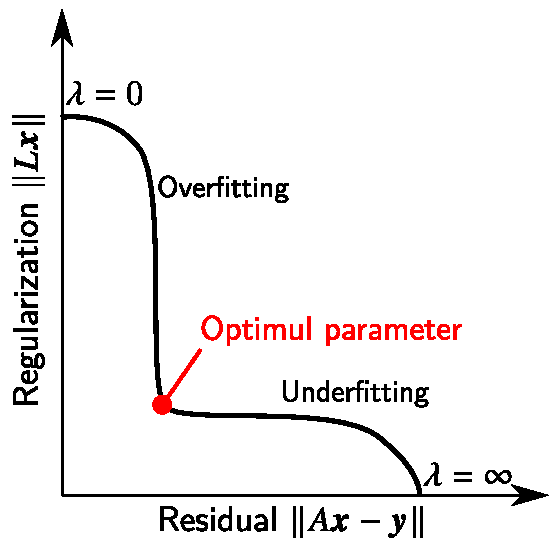
\includegraphics{./regularization/L-curve.pdf}
    \caption{L-curve の概形}
    \label{fig:regularization_l-curve_l-curve}
\end{figure}

正則化の式 \eqref{eq:regularization_intro_general-regularization} を最小化する
$\bm{x}$ を $\bm{x}_\lambda$ として,
横軸を残差 $\|A\bm{x}_\lambda-\bm{y}\|$,
縦軸を正則化項 $R(\bm{x}_\lambda)$ とし,
正則化パラメータ $\lambda$ を変えたときの
プロットを L-curve と呼ぶ.
L-curve は一般に図 \ref{fig:regularization_l-curve_l-curve} のような L の字を
描いている場合が多い.
単純にノルムをプロットするよりも
両対数グラフにプロットする方が
後述する曲線の特徴をはっきりさせられる他,
スケールの違いによる影響を
抑えられるなどのメリットもあるという
\cite{Hansen1998}.

図 \ref{fig:regularization_l-curve_l-curve} のように L-curve が得られた場合,
L の字の曲がり角にあたる赤い点の部分から左上の方では
残差がほとんど減らずに正則化項が増加しており,
右下の方では正則化項がほとんど減らずに残差が増えているため,
両方のバランスが取れている L の字の曲がり角を取るのが良いと考えられる.
そこで,L-curve の曲がり角を数値的に求める手法について考える.

ここでは,文献 \cite{Hansen1998} に従い次の関数の組を考える.
\begin{equation}
    (\xi(\lambda), \eta(\lambda))
    =(\log\|A \bm{x}_\lambda - \bm{y}\|, \log{R(\bm{x})})
\end{equation}
L-curve の曲がり角は曲線 $(\xi(\lambda), \eta(\lambda))$ の
曲率が最も大きい部分と考えられるため,曲率
\begin{equation}
    \kappa(\lambda) =
    \frac{\xi'\eta'' - \xi''\eta'}
    {\left( (\xi')^2 + (\eta')^2 \right)^{3/2}}
\end{equation}
を求め,それを最大化する.
曲率が何らかの手法で求まれば,
1 変数の最適化については
\ref{chap:opt_one-dim-section-search} 章で説明しているため,
ここでは曲率の計算法について考える.
